%%%%%%%%%%%%%%%%%%%%%%% file template.tex %%%%%%%%%%%%%%%%%%%%%%%%%
%
% This is a template file for the LaTeX package SVJour2 for the
% Springer journal "Machine Vision and Applications".
%
%                                    Springer Heidelberg 2004/11/04
%
% Copy it to a new file with a new name and use it as the basis
% for your article. Delete % as needed.
%
%%%%%%%%%%%%%%%%%%%%%%%%%%%%%%%%%%%%%%%%%%%%%%%%%%%%%%%%%%%%%%%%%%%

%s
\documentclass[twocolumn,fleqn,runningheads]{template/svjour2}[23.12.1232]
%
\smartqed  % flush right qed marks, e.g. at end of proof
%
\usepackage{graphicx}
\usepackage{template/biograph}        % to allow for author biography at the end
%
% \usepackage{mathptmx}      % use Times fonts if available on your TeX system
%
% insert here the call for the packages your document requires
%\usepackage{latexsym}
% etc.
%
% please place your own definitions here and don't use \def but
% \newcommand{}{}
%
\journalname{Methoden des maschinellen Lernens}
%
\begin{document}

\title{A machine learning based approach of estimating water intake with inertial sensors}

\author{Cem Basoglu}

\institute{Cem Basoglu \at
           Univ. of Appl. Sci., Minden, Germany \\
		   \email{cem.basoglu@fh-bielefeld.de}
}

\date{Submited: 07/11/2018}

\maketitle

\begin{abstract}
Abstract goes here
\keywords{machine learning \and water intake \and activity recognition \and feature extraction}
\end{abstract}

\section{Introduction}
The consumption of water is crucial for human survival. In order to compensate the loss of water through normal activities, an average person has to consume about 2 to 4.5 litres of water per day under typical climatic conditions \cite{doi:10.1080/02508069608686494}. The long-term low intake of water can lead to various health problems. But managing water intake in everyday life can be a hard and challenging task. The influence of time pressure, stress or in particular the mental state of elderly people, makes it difficult to remember to drink enough.

To support in such situations, there are several approaches using a microphone, to correlate swallowing sounds with the amount of water \cite{7031280,8229307}. While these approaches are producing results with a precision around 10 millilitres, they require the usage of a microphone around the neck. This reduces the user experience and increases the acceptance threshold to use such systems in a continuously way. But the latter one is crucial for accurate estimating of water intake on a daily basis. 

In this paper we examine various machine learning based approaches by using a 3-axis inertial measurement unit attached to the bottle, to estimate the water intake during the day. The base for these approaches is build by the labeled raw data of the accelerator and gyroscope sensors. To collect this learning data, an embedded development board consisting of a micro controller, a Bluetooth Low Energy module and an integrated inertial sensor is used. For the labeling process a mobile application is developed, which leverages the Bluetooth connection to the embedded device and manually records and labels the water intake events. In the next step the data is analyzed to find significant features for spotting water intake events.
\section{Related work}
Amft, O. et al. \cite{5470653} are describing a system based on a wrist-worn inertial sensor to spot drinking motions with an accuracy of 94\%. An additional magnetic coupled sensor attached to the shoulder is used to determine the relative position of the wrist-worn sensor and thereby to recognize the type fluid container and the remaining fluid level with a accuracy of 75\% respectively 72\%. The spotting of motions is based on a feature similarity search using euclidean distance and uses 20 features generated out of the raw sensor data.\\
In \cite{7038937} Dong, B. et al. are also using an inertial sensor to \\
\cite{7031280} \cite{8229307}
\section{Volume estimation}
\begin{figure}
\centering
  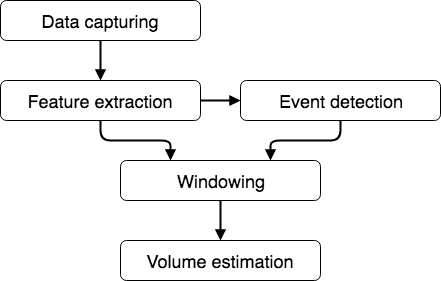
\includegraphics[width=0.45\textwidth]{assets/workflow.png}
\caption{Processing for event spotting and volume estimation}
\label{fig:workflow}
\end{figure}
The accurate and consistent monitoring of water intake depends primarily on continuous usage of a tracking device. To accomplish this, the proposed method aims to reduce the resource requirements in order to perform the event spotting and volume estimation in low power environments. This allows the execution of the application entirely on a constrained device while the smart phone is solely used for interaction. As a result, the monitoring can be performed by the device itself, even when no smart phone is connected.\\
Like depicted in Figure \ref{fig:workflow}, the whole process of event detection and volume estimation is divided into multiple steps. The data flow between the steps is enriched with further information in each step in order to finally estimate the water volume. The actions taken in these steps are described in detail in the following section.


\subsection{Data capturing and feature extraction}
To simplify the collecting and labeling process of training data, a mobile application has been developed that connects to the Intel Curie development board \cite{Supportf64:online} through BLE and records the inertial sensor data at 25 Hz. In this process a total of 40 events were collected, of which 27 are water intake events and 13 represent noise. The data read from the inertial sensor consists of the acceleration and angular velocity values in the three dimensional axes. Since there is a strong correlation between the axes of the accelerometer and the two horizontal (x, z) axes of the bottle depend on the rotation around the y-axis of the bottle, only the vertical y-axis is used for the estimation. The rotation of the bottle also affects the gyroscope, which is why only the magnitude of the vector is used in the volume estimation process.\\

\begin{equation}
||magnitude|| = \sqrt{x^2+y^2+z^2}    
\end{equation}
Figure \ref{fig:features} depicts a typical water intake event, using accelerometer value which corresponds to the y-axis of the bottle and the magnitude of the gyroscope. 

\begin{figure}
\centering
  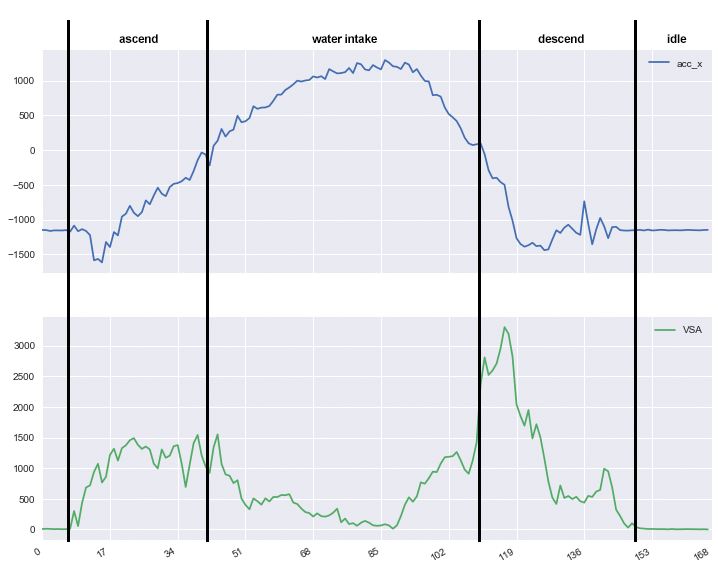
\includegraphics[width=0.45\textwidth]{assets/features.png}
\caption{Features for event detection and volume estimation}
\label{fig:features}
\end{figure}

\subsection{Event detection}

\begin{figure}
\centering
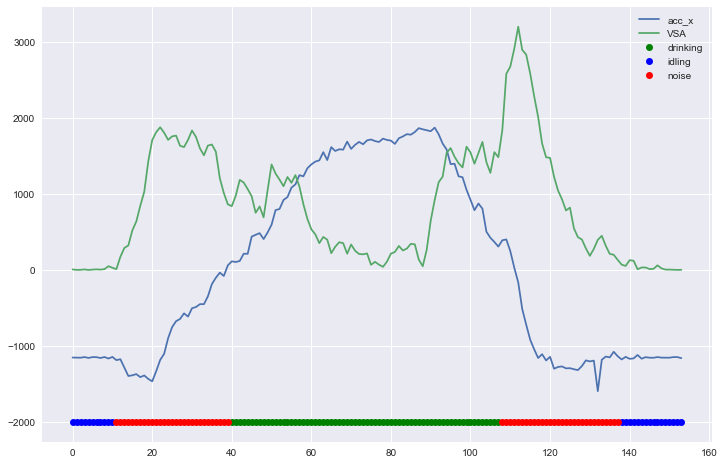
\includegraphics[width=0.48\textwidth]{assets/spotting.png}
\caption{Hidden states of event detection}
\label{fig:hidden_states}
\end{figure}

In this step of the volume estimation process the extracted features are used to inference the phases of a drinking process. As depicted in Figure \ref{fig:features}, a drinking process consists of the phases: idle, ascend/descend and water intake. The water intake phase is the actual phase of interest and is required in the subsequent steps of the estimation process. Furthermore, the start and the end of the phase is required for an accurate volume estimation. This means it is not sufficient to measure the similarity between time series with algorithms such as dynamic time warping (DTW). As described by Esmael, B. et al. in \cite{Bagnall2017}, it requires methods which take the different phases of the time series into account. One of those methods is the Hidden Markov Model (HMM), a statistical model with hidden states to represent the phases during the classification process \cite{6421385}. This classifier has a relatively low computational complexity during the inference phase and satisfies the requirement to run on restricted devices. 
The HMM is trained with the collected data and extracted features described in the previous step. For the selection of the model parameters, various combinations of the parameters listed in Table \ref{tab:score} were considered and scored with the logarithmic likelihood function. 
\begin{table}[h]
    \centering
    \caption{Model parameters and score}
    \begin{tabular}{lcr}
        \hline\noalign{\smallskip}
        covariance type     &   hidden states   & log likelihood \\
        \tableheadseprule\noalign{\smallskip}
        spherical           &   2               & -81734.595809 \\
        diagonal            &   2               & -80969.464356 \\
        full                &   2               & -80183.335626 \\
        spherical           &   3               & -76584.218748 \\
        diagonal            &   3               & -76097.221068 \\
        full                &   3               & -75791.043781 \\
        diagonal            &   4               & -74546.967384 \\
        full                &   4               & -74290.390349 \\
        spherical           &   4               & -74194.977340 \\
        \noalign{\smallskip}\hline
    \end{tabular}
    \label{tab:score}
\end{table}\\
Although a model trained with a single variance value for each state (spherical) and 4 hidden states has the maximum likelihood (see Table \ref{tab:score}), the model trained with only 3 hidden states and a covariance matrix for each state achieves better results during cross validation with the test data. The colored line at the bottom of the plot in Figure \ref{fig:hidden_states}, represents the 3 hidden states inferred from the extracted features of the previous step and correspond with the phases of the drinking process described above.


\subsection{Windowing and volume estimation}
\begin{figure}
\centering
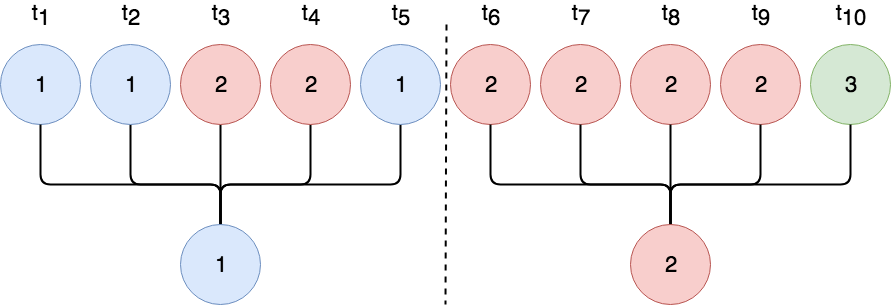
\includegraphics[width=0.4\textwidth]{assets/windowing.png}
\caption{Majority window filter}
\label{fig:windowing}
\end{figure}
For estimating the volume, the inferred state of the previously described step and the value of the acceleration sensor for the y-axis of the bottle are used. Since these values are processed at 25 Hz in the previous steps, the deviation between the volume estimation and the water actually consumed increases. To minimize this estimation error and smooth the state transitions, these values are windowed, which also results in a lower sampling rate. In the case of event detection, a majority window filter (see Figure \ref{fig:windowing}) is used and only the major inferred state in the window is forwarded. For the values of the accelerometer a moving average filter is applied. The window size for both filters takes 5 values for each window without overlapping, which results in a sampling rate of 5 Hz.\\

In the volume estimation step the inferred state acts as an activation gate for the estimating function. If the inferred state corresponds with the drinking phase of the drinking process depicted in Figure \ref{fig:hidden_states}, the following function is used to estimate the water intake.
\begin{equation}
volume = \sum\limits_{i=1}^n \bigg(normalize(acc\_x_i) * c \bigg)
\end{equation}
Each value from the acceleration sensor is normalized and multiplied with a constant value to estimate the total volume of the water intake event. The normalization of the accelerometer value is required to produce values between 0 and 1 and acts as a weight for the constant value. The value $c$ represents the volume for a single signal from the windowing step and is calculated by using the total volume of each water intake event collected during the development phase of the proposed method.
\begin{equation}
c = \frac{\sum\limits_{j=1}^{m}volume_j}{\sum\limits_{j=1}^{m}\sum\limits_{i=1}^n normalize(acc\_x_{ji})}
\end{equation}
In order to determine the constant value $c$, a total of 15 water intake events and the corresponding volumes are evaluated. The outer sum counting from the indices j to m of the above formula, represents each water intake event while the inner sum corresponds to accelerometer values of a single water intake event. The numerator is the total volume of each water intake event and the denominator the sum of all accelerometer values. In comparison to other machine learning methods with regression models for estimation of water intake volume, the presented method is very lightweight and has a relatively low computational complexity in order to satisfy requirements described in the introduction of this chapter.

\section{Experimental Results}
\section{Conclusion}




\bibliographystyle{template/spmpsci.bst}
\bibliography{0_bibliography}

\end{document}
% end of file template.tex
